% !TEX program = xelatex
\documentclass[11pt]{beamer}

\usepackage{unicode-math}
\usepackage{amsmath}
\usepackage{amsfonts}
\usepackage{amssymb}
\usepackage[style=ddmmyyyy]{datetime2}
\usepackage{graphicx}
\usepackage{hyperref}
\usepackage{fontspec}

\makeatletter
\def\input@path{{../../theme/}}
\makeatother

%beamer setup
\usetheme[subsectionpage=progressbar]{mis}
\setbeamerfont{caption}{size=\footnotesize}
\setsansfont{Lato Semibold}[Numbers=OldStyle]
\setmathfont{STIX Two Math}[Scale=MatchLowercase]
\setmonofont{Consolas}[Scale=MatchLowercase]


\author{Lê Thành Văn}
\title{Các dạng chuẩn của CSDL quan hệ}
\institute{Khoa Hệ thống thông tin quản lý}
\date{\today}
\hypersetup {
	colorlinks = true
}
%\usecolortheme{seahorse}
% graphic path
\graphicspath{{../../media/}}

\renewcommand{\figurename}{Hình}
%
\AtBeginSection{
  \frame{
    \sectionpage
  }
}
\begin{document}
\begin{frame}
  \titlepage
\end{frame}

\section{Giới thiệu}
\subsection{Định nghĩa}
\begin{frame}
  Chuẩn hóa cơ sở dữ liệu (csdl) là quá trình tách bảng dữ liệu nhằm:
  \begin{itemize}
    \item giảm thiểu việc dư thừa dữ liệu, và
    \item hạn chế lỗi có thể phát sinh trong quá trình thay đổi dữ liệu.
  \end{itemize}
\end{frame}

\begin{frame}
  Việc chuẩn hóa csdl dựa trên các dạng chuẩn (normal form) được Edgar F. Codd
  đề ra trong mô hình quan hệ của mình.
\end{frame}
\subsection{Các loại lỗi}
\begin{frame}
  \textbf{Lỗi khi thay đổi dữ liệu} (thêm, sửa hoặc xóa) là dạng lỗi khi dữ liệu được thay đổi không tương thích 
  với cấu trúc hoặc dữ liệu hiện có.
\end{frame}

\begin{frame}
  Giả sử thông tin giảng viên \textit{cần} bao gồm mã môn học họ giảng dạy.
  Tuy nhiên, một giảng viên mới có thể chưa có môn, dẫn đến không thể thêm thông tin của họ.

  \begin{figure}
    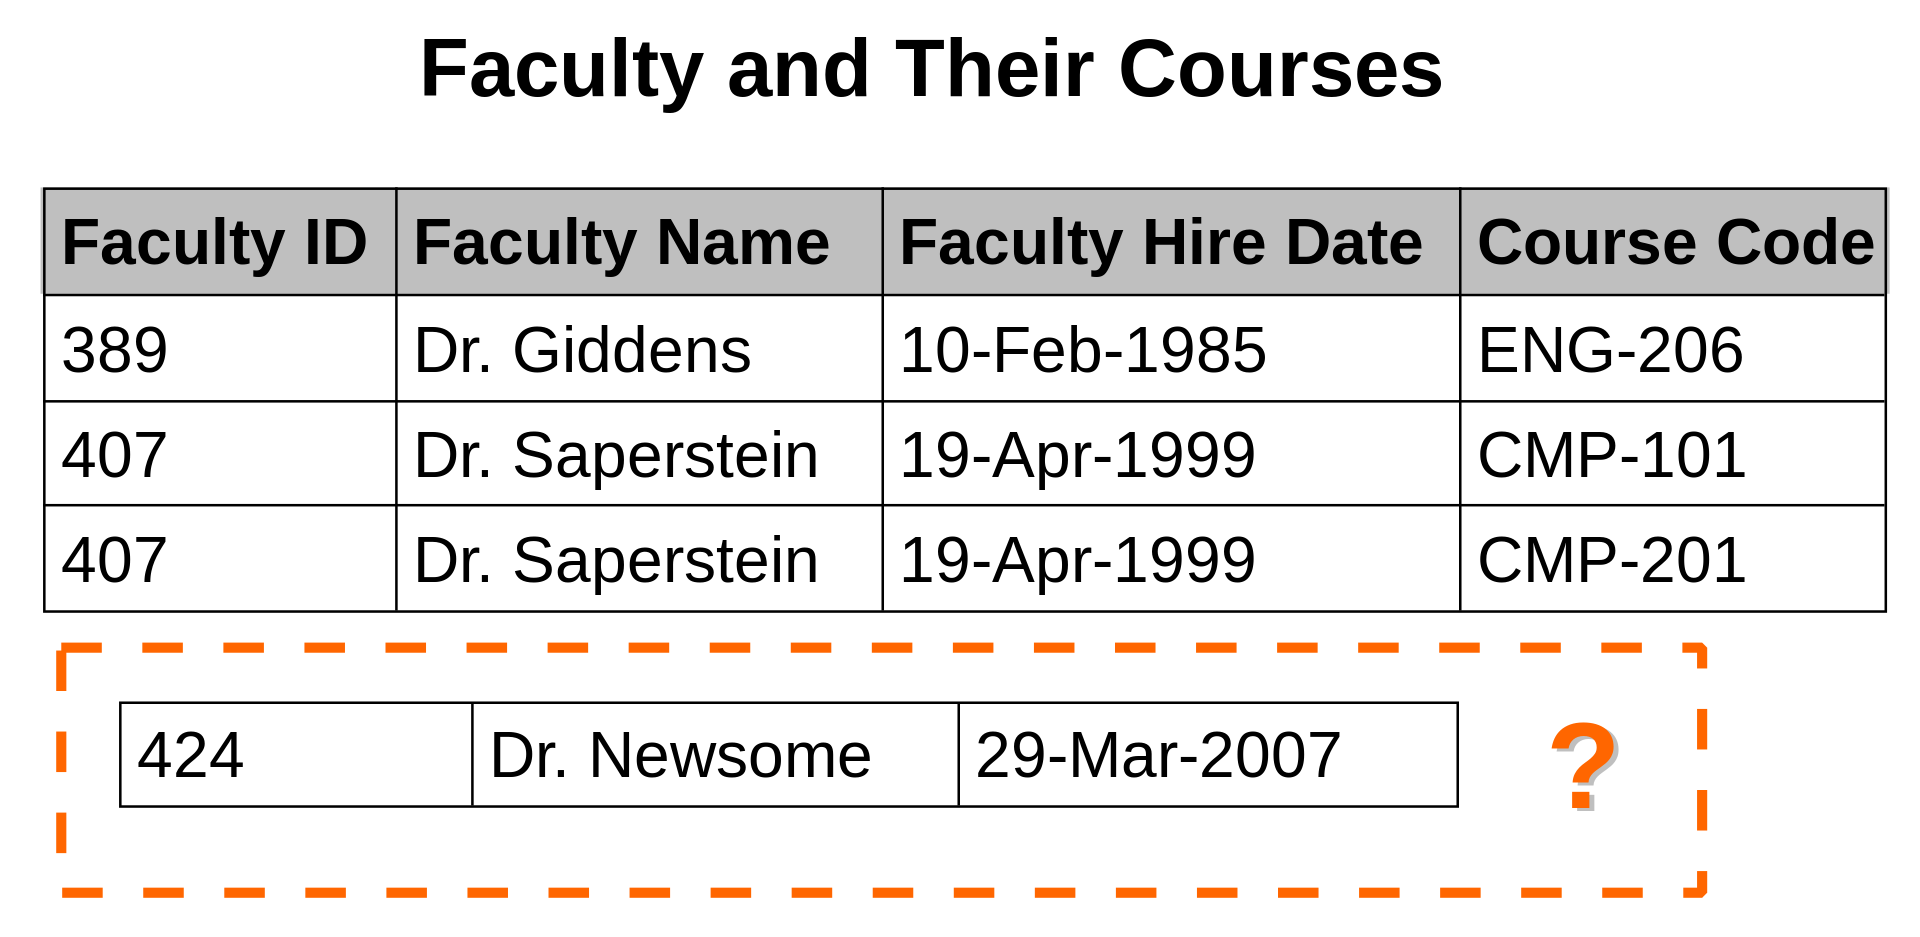
\includegraphics[width=0.75\textwidth]{COS212/ia.png}
    \caption{\textit{Lỗi khi thêm dữ liệu}}
  \end{figure}
\end{frame}

\begin{frame}
  Một thông tin có thể xuất hiện nhiều lần trong một bảng, nên khi thay đổi có thể bị sót, 
  dẫn đến thông tin không nhất quán trong csdl.
  \begin{figure}
    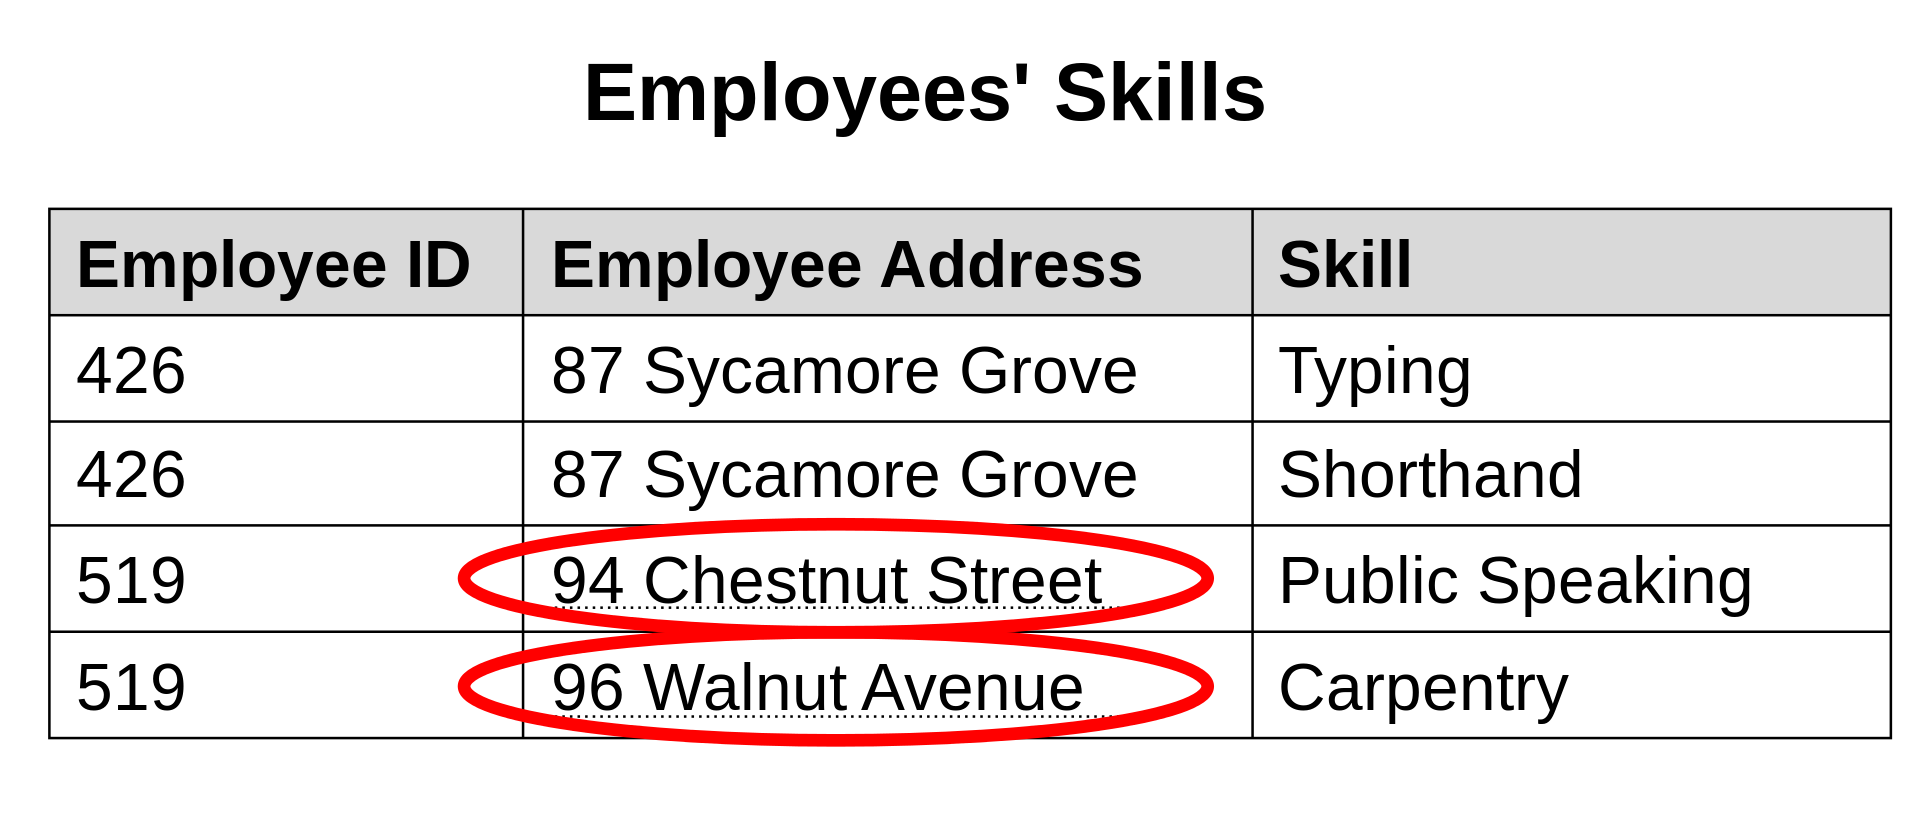
\includegraphics[width=0.75\textwidth]{COS212/ua.png}
    \caption{\textit{Lỗi khi sửa dữ liệu}}
  \end{figure}
\end{frame}

\begin{frame}
  Lỗi khi xóa dữ liệu là dạng lỗi mà khi xóa một thông tin này có thể xóa những 
  thông tin (không cần xóa) khác.
  \begin{figure}
    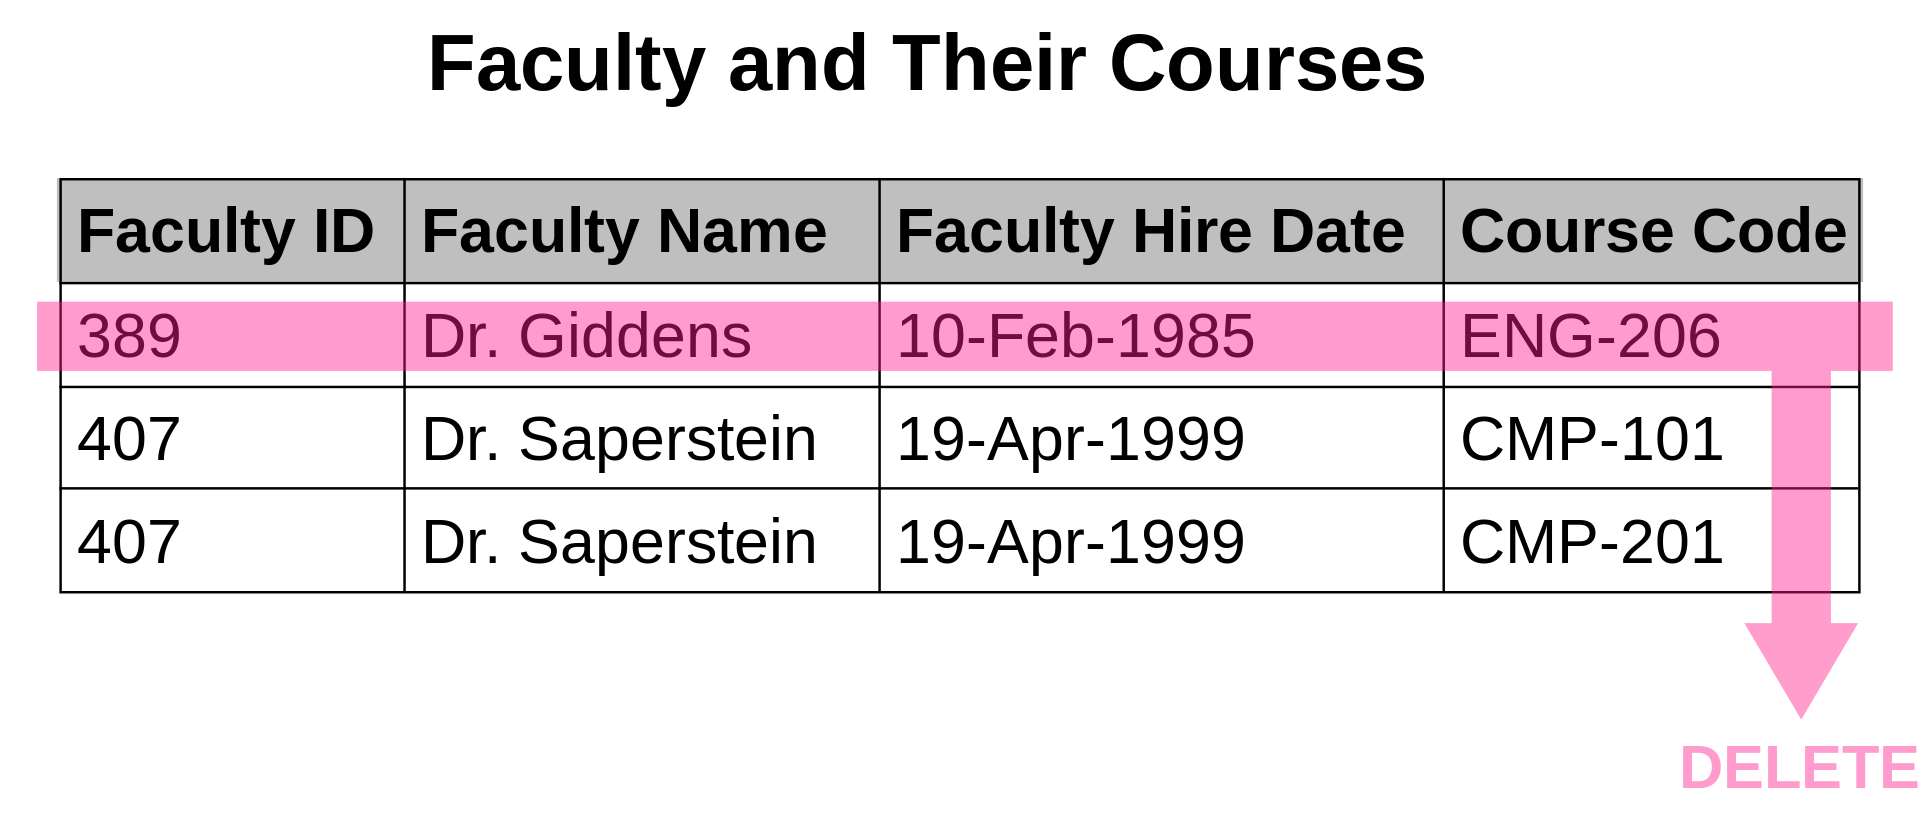
\includegraphics[width=0.75\textwidth]{COS212/da.png}
    \caption{\textit{Lỗi khi xóa dữ liệu}}
  \end{figure}
\end{frame}

\subsection{Các dạng chuẩn}
\begin{frame}
  Các dạng chuẩn thường gặp bao gồm (từ thấp đến cao):
  \begin{itemize}
    \item Dạng chuẩn 1 (First Normal Form, 1NF).
    \item Dạng chuẩn 2 (Second Normal Form, 2NF).
    \item Dạng chuẩn 3 (Third Normal Form, 3NF).
    \item Dạng chuẩn Boyce-Codd (Boyce-Codd Normal Form, BCNF, 3.5NF). 
  \end{itemize}
\end{frame}

\begin{frame}
  Việc đạt được một dạng chuẩn cao có nghĩa là phải thỏa mãn điều kiện của các dạng chuẩn thấp hơn nó.\\
  Tức là, không thể đạt được dạng chuẩn 3 nếu như không đạt được dạng chuẩn 1 hoặc dạng chuẩn 2.
\end{frame}

\begin{frame}
  Một csdl quan hệ được gọi là \textbf{đã chuẩn hóa} nếu như nó đạt được dạng chuẩn 3.
\end{frame}
\end{document}